



\section{Application to protoplanetary disks}\label{linear_problem}
We now examine instabilities in dusty protoplanetary disks
based on explicit descriptions of the equilibrium state. We first
specify the disk structures to be analyzed. We show  
that sharp radial edges in the dust-to-gas ratio can render the disk unstable. We then 
revisit two well-known instabilities in dusty gas using the
hydrodynamic framework developed thus far, namely secular gravitational (SGI) 
instabilities and the streaming instability (SI).  

\subsection{Disk structure with a prescribed dust distribution}\label{steady_state}  
We assume a Gaussian profile in the
dust-to-gas ratio,    
\begin{align}\label{dust_gauss}
  \epsilon(r,z) = \epsilon_0(r)
  \exp{\left[-\frac{z^2}{2\Htilde^2(r)}\right]}. 
\end{align}
%For simplicity we assume the dust-to-gas ratio at the mid-plane
%$\epsilon_0$, as well as its characteristic scale-height
%$\widetilde{H}$, are both constant.
% We take the mid-plane dust-to-gas ratio
%to be a power-law in radius,  
%\begin{align}
%  \epsilon_0(r) = \epsilon_{00}\left(\frac{r}{r_0}\right)^{-d},  
%\end{align}
%where $\epsilon_{00}$ is the dust-to-gas ratio at the fiducial radius
%$r_0$.  
Inserting Eq. \ref{dust_gauss} into vertical hydrostatic equilibrium,
Eq. \ref{steady_momz} and integrating with the approximate
gravitational potential (Eq. \ref{thin_disk_potential}) we obtain the
gas density as
\begin{align}
  &\rhog(r,z)= \notag\\
&\rho_\mathrm{g0}(r)\exp{\left\{ - \frac{z^2}{2\Hgas^2}
    -\epsilon_0\frac{\Htilde^2}{\Hgas^2}\left[1 -
      \exp{\left(-\frac{z^2}{2\Htilde^2}\right)}\right] \right\}}, 
\end{align}
where
\begin{align}
  \Hgas = \frac{c_s}{\OmK}, \quad \OmK \equiv \sqrt{\frac{GM_*}{r^3}},   
\end{align}
is the gas scale-height in the dust-free limit and $\OmK$ is the
Keplerian frequency, respectively. 

In gas-dominated disks with $\epsilon_0 < 1$ the gas distribution
$\rhog(r,z)$ is close to Gaussian, as in the   
dust-free case, and the dust density is approximately 
\begin{align}
  \rhod \simeq \epsilon_0\rho_\mathrm{g0}(r) \exp
        {\left(-\frac{z^2}{2H_\mathrm{d}^2}\right)}, 
\end{align}
with 
\begin{align}
  \frac{1}{H_\mathrm{d}^2} = \frac{1}{\Htilde^2} + \frac{1}{\Hgas^2}, 
\end{align}
and $H_\mathrm{d}$ is the dust-scale height.% In numerical
%calculations, we  we specify $H_\mathrm{d}< \Hgas$ to obtain 
%$\Htilde$ for input. 

Finally, we define 
\begin{align}
  Z \equiv \epsilon_0\frac{\Hd}{\Hg} \simeq
  \frac{\Sigma_\mathrm{d}}{\Sigma_\mathrm{g}} 
\end{align}
as a measure of the local metalicity, where $\Sigma_\mathrm{d}$ and
$\Sigma_\mathrm{g}$ are the dust and gas surface densities,
respectively. The second equality holds for $\epsilon_0\ll1$.  

%\Sigma_\mathrm{d}$ and the gas
%surface density $\Sigma_\mathrm{g}$.  

\subsubsection{Orbital frequency} 
From Eq. \ref{steady_momr} the disk orbital frequency is 
\begin{align}
  \Omega(r,z) = \OmK(r)\left[1 - \frac{3}{2}\frac{z^2}{r^2} +
    \frac{h_\mathrm{g}^2}{\left(1+\epsilon\right)}\frac{\p}{\p\ln{r}}\ln{\left(c_s^2\rhog\right)}
    \right]^{1/2}, 
\end{align}
where 
\begin{align}
  h_\mathrm{g} \equiv \frac{\Hgas}{r}
\end{align}
is the characteristic disk aspect-ratio, with $h_\mathrm{g}\ll 1$ for protoplanetary disks. 

\subsubsection{Vertical shear}\label{vertshear}
Writing Eq. \ref{vshear} in terms of the gas density and dust-to-gas
ratio with a power-law temperature profile (Eq. \ref{power_temp})
gives the disk's explicit vertical shear profile:
\begin{align}\label{vshear2}
  &r\frac{\p \Omega^2}{\p z}  =
  \frac{c_s^2(r)}{\left(1+\epsilon\right)^2}\left\{
  \frac{\p\epsilon}{\p r}\frac{\p\ln{\rhog}}{\p z}
%  -\frac{\p\epsilon}{\p z}\left[\frac{\p\ln{\rhog}}{\p r} + \frac{q}{r}\right]\right.\notag\\
 -\frac{\p\epsilon}{\p z}\frac{\p\ln{P}}{\p r}\right.\notag\\
  &\phantom{ r\frac{\p \Omega^2}{\p z}  =
    \frac{c_s^2(r)}{\left(1+\epsilon\right)^2}\left\{\right\} }
  \left. -\frac{q}{r} \left(1+\epsilon\right)\frac{\p\ln{\rhog}}{\p z}
  \right\}. 
\end{align}
The first two terms correspond to vertical shear caused by spatial
variations in the dust-to-gas ratio. The third term
proportional to $q$ corresponds to vertical shear due to the 
radial temperature gradient, which survives in the dust-free limit. 

We can compare these sources by 
evaluating them using the equilibrium
solutions in \S\ref{steady_state}. We assume the disk is radially
smooth so that $\p_r\sim 1/r$. % and the dust-to-gas ratio
% $\epsilon\ll1$. 
This gives 

\begin{align}\label{vshear_split}
  \frac{\left|r\p_z\Omega\right|_{\text{
        dust/gas gradient}}}{\left|r\p_z\Omega\right|_{\text{
        temp. gradient}}} \sim
 % \epsilon \frac{\mathrm{max}\left(\delta^2,
  %  1\right)}{\left|q\right|\left(\epsilon + \delta^2\right)},
 \epsilon \frac{\mathrm{max}\left(\delta^2,
    1\right)}{\left|q\right|\left(1+\epsilon\right)\delta^2},
\end{align}
where $\delta\equiv \Htilde/\Hgas$. 
Since $|q|=O(1)$ in PPDs, Eq. \ref{vshear_split} indicates that
vertical shear due to variations in the dust-to-gas ratio dominates 
over that due to the radial temperature gradient for thin dust layers
such that $\delta^2\ll \epsilon$. %Otherwise, vertical shear is
%associated with the radial temperature gradient. %However, axisymmtric
%\emph{instability} always caused by $\p_rc_s^2$.  






\subsubsection{Dusty vertical buoyancy}\label{vbuoyancy}
For the above equilibrium the vertical buoyancy frequency is given
explicitly as 
\begin{align}
  N_z^2 =
  %\frac{c_s^2(r)}{\left(1+\epsilon\right)^2}\frac{\p\ln\rhog}{\p 
%  z}\frac{\p\epsilon}{\p z} \\ &
  %                                =
 \frac{\epsilon}{\left(1+\epsilon\right)^2}\left(\frac{z}{\Htilde}\right)^2\OmK^2\notag,  
\end{align}
where we have used $c_s=c_s(r)$. Then 
\begin{align*}
N_z\lesssim
O\left(\sqrt{\epsilon_0}\OmK\right). 
\end{align*}
However, for well-mixed dust layers such that $H_\epsilon \gg \Hg$, 
$\mathrm{max}\left(N_z\right)$ may occur outside a finite vertical domain.  

\subsection{Instability of dusty edges} 
Here we apply the dusty analog of the Solberg-Hoiland criteria derived
in \S\ref{iso_perfect} assuming strictly isothermal gas. As discussed
there, the first criterion is generally satisfied. Thus we only
consider the second condition, Eq. \ref{dusty_solberg2}.  

We assume the disk is approximately Keplerian so that
$\kappa\simeq\OmK$, and that the vertical gas distribution is   
Gaussian. In terms of the dust-to-gas
ratio $\epsilon$, Eq. \ref{dusty_solberg2}
becomes 
\begin{align}
  % &1 + \frac{\epsilon}{\left(1+
  %   \epsilon\right)^2}\left(h_\mathrm{g}^2\frac{\p\ln{\rhog}}{\p\ln{r}}
  % \frac{\p\ln{\epsilon}}{\p\ln{r}} + 
  % \frac{z^2}{\Htilde^2}\right)>0 \label{stability_est1},   \\ 
% &1 - \frac{\epsilon
%   h_\mathrm{g}^2}{\left(1+\epsilon\right)^2}
%   \frac{\p\ln{\epsilon}}{\p\ln{r}}\left(-\frac{\p\ln{\rhog}}{\p\ln{r}}+\frac{\Htilde^2}{H_\mathrm{g}^2}\frac{\p\ln{\epsilon}}{\p\ln{r}}\right)
%   > 0 \label{stability_est2},
&1 - \frac{\epsilon
  h_\mathrm{g}^2}{\left(1+\epsilon\right)^2}
  \frac{\p\ln{\epsilon}}{\p\ln{r}}\left(-\frac{\p\ln{P}}{\p\ln{r}}+\frac{\Htilde^2}{H_\mathrm{g}^2}\frac{\p\ln{\epsilon}}{\p\ln{r}}\right)
  > 0 \label{stability_est2},
\end{align}
for \emph{stability}. The { first term in  brackets} is usually stabilizing in 
PPDs for reasons given in \S\ref{iso_perfect}. The { second term in
brackets} is 
always destabilizing, but is small in smooth, thin disks with radial
gradients $O(1/r)$, $h_\mathrm{g}\ll 1$, 
provided that $H_\epsilon/\Hg$ is not large (e.g. some dust settling
has occurred). This means that typical dusty PPDs are stable to
axisymmetric perturbations, even for arbitrarily thin
dust layers. 

%%%%%%%%%%%%%%%%%%

To violate Eq. \ref{stability_est2} and obtain instability, notice the 
left hand side is a quadratic in $\p_r\epsilon$. Thus instability is possible for
sufficiently large (in magnitude) radial gradients  in the dust-to-gas
ratio,  
\begin{align}
  \frac{\p\ln{\epsilon}}{\p\ln{r}} > \chi_+ \quad \mathrm{or} \quad 
  \frac{\p\ln{\epsilon}}{\p\ln{r}} < \chi_-,
\end{align}
for \emph{instability}, where
\begin{align}\label{spm}
% \chi_\pm = \frac{1}{2}\frac{H_\mathrm{g}^2}{\Htilde^2} 
%   \left[
%   \frac{\p\ln{\rhog}}{\p\ln{r}} \pm 
%   \sqrt{
%   \left(\frac{\p\ln{\rhog}}{\p\ln{r}}\right)^2 + 
%   4 \frac{\Htilde^2}{H_\mathrm{g}^2}
%   \frac{\left(1+\epsilon\right)^2}{\epsilon h_\mathrm{g}^2}
%   }
%   \,\right]. 
\chi_\pm = \frac{1}{2}\frac{H_\mathrm{g}^2}{\Htilde^2} 
  \left[
  \frac{\p\ln{P}}{\p\ln{r}} \pm 
  \sqrt{
  \left(\frac{\p\ln{P}}{\p\ln{r}}\right)^2 + 
  4 \frac{\Htilde^2}{H_\mathrm{g}^2}
  \frac{\left(1+\epsilon\right)^2}{\epsilon h_\mathrm{g}^2}
  }
  \,\right]. 
\end{align} 
In typical accretion disks where $\p_rP<0$, instability is easier
for increasing dust-to-gas ratios ($\p_r\epsilon > 0$).  

We can neglect pressure gradients in Eq. \ref{spm} 
if $r\p_r\ln{P}\sim O(1)$ and $H_\epsilon/\Hgas\gg
\sqrt{\epsilon}\hgas/2\left(1+\epsilon\right)$. For example, if $\epsilon\simeq 0.01$ and
$\hgas\simeq 0.05$, then we require $H_\epsilon/\Hg\gg
2\times10^{-3}$. This can be met if the dust is not well settled { (e.g. due to a small amount of turbulence).}  
%this turbulence cannot be too big because the analysis itself does not have diffusion/turbulence 
%large diffusion is expected to stabilize 
Then instability requires 
\begin{align}\label{dust_edge}
\left|\frac{\p\ln{\epsilon}}{\p r}\right| \gtrsim
  \frac{1}{\Htilde}\frac{\left(1+\epsilon\right)}{\sqrt{\epsilon}}.
%\simeq
 % \frac{1}{\sqrt{\epsilon}H_\epsilon}, 
\end{align}
%where the second equality applies to $\epsilon\ll 1$. 
That is, if the radial lengthscale of the dust-to-gas ratio 
is much less its vertical lengthscale, $L_\epsilon\ll O(\Htilde)$, 
then the system is  unstable.  
Taking $\epsilon\sim 0.01$,  we find that 
for thin dust layers with $H_\epsilon \simeq \Hd\ll \Hg$,  instability
requires $L_\epsilon\ll O(0.1\Hg)$, i.e. the dust-to-gas ratio must 
vary on an extremely short radial lengthscale. This might be achieved, for
example, at sharp edges associated with gaps opened by giant planets. 

Technically, the above discussion is only applicable when $c_s$ is
constant and $\tstop=0$ (see \S\ref{iso_perfect}). However, since
dusty edges translate to sharp entropy gradients (
\S\ref{dusty_entropy}), we may generally expect sharp features in the
dust distribution of protoplanetary disks to be unstable.    


%{\bf mention this is equivalent to sharp entropy gradients?}

\subsection{Radially local problem}
We now specialize further and compute explicit solutions to the linear
problem. We consider radially-localized axisymmetric disturbances of the form  
\begin{align}
  \delta X (r, z) = \delta X_1(r,z)\exp{(\ii k_x r)},
\end{align} 
%and similarly for $\dd P$ and $\dd\bm{v}$. 
where $k_x$ is a real wavenumber such that $|k_xr|\gg 1$, and the 
amplitude $\dd X_1(r,z)$ is 
a slowly-varying function of $r$. Then 
$\p_r\to i k_x$ when acting on the above primitive perturbations, and we may
neglect curvature terms. We take  
$k_x>0$ without loss of generality. Hereafter, we drop the subscript 1
on the amplitudes. 
%The frequency $\sigma = \omega +
%\ii s$ is generally complex, with $\omega$ being the real frequency
%and $s$ is the real growth rate. 

Introducing 
\begin{align}
  W \equiv \frac{\dd\rho}{\rho}, \quad Q \equiv \frac{\dd P}{\rho},
\end{align}
the linearized equations for 
vertically isothermal dusty gas with the pressure
equation in place of the dust-fraction
(Eq. \ref{masseq}, \ref{momeq}, \ref{poisson}, \ref{eff_energy}) are then:    

\begin{align}
  \ii\sigma W &= \ii k_x \dd v_r + \dd v_z^\prime +
  \dd v_r \p_r\ln{\rho} + \dd v_z\p_z\ln{\rho},\label{lin_mass}\\
  -\ii\sigma\dd v_r  &= 2\Omega\dd v_\phi 
% +  \delta\bm{F}\cdot\hat{\bm{r}}
- W F_r - \ii k_x Q - \ii k_x\dd\psi,\label{lin_xmom}\\
  \ii\sigma\dd v_\phi &= \frac{\kappa^2}{2\Omega}\dd v_r + \frac{\p
    v_\phi}{\p z}\dd v_z, \label{lin_ymom}\\
  -\ii\sigma\dd v_z &= - W F_z - \left[Q^\prime + Q
    \left(\ln{\rho}\right)^\prime\right] - \dd\psi^\prime  %\delta\bm{F}\cdot\hat{\bm{z}} 
,\label{lin_zmom}\\
  \ii\sigma Q &= \frac{P}{\rho}\left(\ii k_x \dd v_r + \dd
               v_z^\prime\right) + \frac{1}{\rho}\left(\dd v_r\p_rP + \dd v_z \p_zP\right)\notag\\
                &\phantom{=}-\frac{P}{\rho} \dd v_r\p_r
               \ln{c_s^2} %, \label{lin_energy} 
%+ \dd v_z \p_z\ln{c_s^2}\right),\label{lin_energy} 
               - \frac{\dd\mathcal{C}}{\rho},\label{lin_energy}\\
\dd\psi^{\prime\prime}  &= 4\pi G \rho W + k_x^2\dd\psi, \label{lin_sg}
\end{align}  
where $^\prime \equiv \p_z$ and recall $\bm{F} \equiv -\nabla
P/\rho$. We have temporarily restored self-gravity  to
discuss SGI in the next
section. The linearized dust-diffusion function 
$\dd\mathcal{C}$ is given in  Appendix \ref{lin_dust}. 
% and $\dd\bm{F}$ is the linearized pressure
%force, given in Appendix \ref{lin_press}. 
%Note that we have assumed a temperature profile that only depends on $r$.   

%; and 
%\begin{align}
%  \delta \bm{F} \equiv \frac{\dd\rho}{\rho^2}\nabla P -
%  \frac{1}{\rho}\nabla\dd P, 
%\end{align}
%$\dd\mathcal{C}$ is the linearized dust-duffusion function, given in
%Appendix \ref{lin_dust}. We consider stopping times appropriate for
%small grains in the Epstein regime. Note that for the axisymmetric
%problem, $\dd\bm{F}$ is purely meridional. 

Eq. \ref{lin_mass}---\ref{lin_sg} is a set of ordinary
differential equations in $z$. All coefficients and amplitudes are
evaluated at a fiducial radius $r=r_0$, but their full $z$-dependence
is retained. We next discuss solutions to these equations.  We first
show that the above equations yield the SGI and SI in the strong
drag regime in \S\ref{sgi} and \S\ref{si}, respectively. We then
consider 3D, stratified disks in \S\ref{results} to study how the addition of  dust 
affects the vertical shear instability. 

%for a
%razor-thin, self-gravitating disk in \S\ref{sgi}; and for 3D
%non-self-gravitating, unstratified and stratified disks 
%in \S\ref{si} and \S\ref{results}, respectively.   
 
 % Numerical solutions are generally required for the 
%vertically-stratified problem. 

%\section{Connection to previous results}



\subsubsection{Secular gravitational instability}\label{sgi}
Consider a razor-thin, self-gravitating disk so that $\rho =
\Sigma\delta(z)$, where $\delta$ is the Dirac delta function and $\Sigma$ is
the total surface density. Here $\epsilon = \Sigma_\mathrm{d}/\Sigma_\mathrm{g}$ and 
$\tepsilon=\Sigma_\mathrm{d}/\Sigma$, where $\Sigma_\mathrm{d,g}$ are the dust and gas surface densities. 
The background disk is 
uniform and we neglect the vertical dimension   
in Eq. \ref{lin_mass}---\ref{lin_energy}. The linearized dust-gas drag
term is then $-\delta\mathcal{C}/\rho = \tstop\tepsilon c_s^2k_x^2
Q$. The thin-disk solution to Eq. \ref{lin_sg} is $\dd\psi(z=0) = -2\pi G
\Sigma W/\left|k_x\right|$.%, where $\Sigma$ is the total surface
%density. 

These simplifications yield the dispersion relation
\begin{align*}
  \left(\ii\sigma - \tstop\tepsilon c_s^2k_x^2\right)\left( 2 \pi G
    \Sigma \left|k_x\right|  - \kappa^2 + \sigma^2 \right) = \ii
  \sigma c_s^2 k_x^2\left(1 - \tepsilon\right). 
\end{align*}
Searching for slowly and purely growing modes, $\sigma = \ii s$ with 
$|s|\ll \kappa$, we find 
\begin{align}  
s = \frac{\tstop\tepsilon c_s^2 k_x^2 \left( 2 \pi \Sigma G
    \left|k_x\right| - \kappa^2\right)}{\kappa^2 -2 \pi \Sigma G
    \left|k_x\right| + c_s^2k_x^2\left(1-\tepsilon\right) }. \label{sgi_disp}
\end{align}
This is secular gravitational instability mediated by strong
dust-gas drag with negligible turbulent dust diffusion 
\citep[][ their Eq. 13 becomes our Eq. \ref{sgi_disp} in this limit
after 
a change of variables]{takahashi14}. A similar effect occurs in viscous
self-gravitating gas disks \citep{gammie96,lin16}. In fact, if we
identify $\nu \equiv \tstop \tepsilon c_s^2$ as a kinematic viscosity,
then Eq. \ref{sgi_disp} is identical to \citeauthor{gammie96}'s Eq. 18. 

This exercise shows that the one-fluid framework, further simplified by
the terminal velocity approximation, is sufficient to capture SGI
in the strong drag limit. 

\subsubsection{Streaming instability}\label{si}
We now consider 3D disks without self-gravity. We neglect the vertical     
component of the stellar gravity, appropriate for studying regions
near the disk midplane. This  
allows us to Fourier analyze in $z$ to obtain 
an algebraic dispersion relation of the form  
$\sum_{j=0}^{5}c_j(k_x,k_z)\sigma^j = 0$, where $k_z$ is a real
vertical wavenumber. The coefficients $c_j$ can be read 
off Eq. \ref{streaming_dispersion} in  Appendix \ref{compressible_streaming}. 
There we also show that this dispersion relation reduces to that for
the streaming instability (SI) in the limit of incompressible gas and small
$\tstop$ \citep{youdin05a,jacquet11}.   
 
%\subsection{Numerical examples}

%{\bf note: kappa2 accounts for dust effect assuming smallh=0.05}

In Table \ref{si_compare} we solve the full dispersion relation
(Eq. \ref{streaming_dispersion}) numerically for selected cases where
analytic SI growth rates have been verified with particle-gas
numerical simulations \citep[namely][]{youdin07b,bai10b}.  
Following previous works on SI, we use normalized 
wavenumbers $K_{x,z} = \eta r k_{x,z}$ where
\begin{align} 
  \eta \equiv -\frac{1}{2\rhog r\OmK^2}\frac{\p P}{\p r} = 
  \frac{1}{2\left(1-\tepsilon\right)}\frac{F_r}{r\OmK^2}, 
\end{align} 
measures the pressure offset of Keplerian rotation. We fix 
$\eta=0.05c_s/r\OmK$. In this section section we also quote the
particle stopping time $\tau_\mathrm{s}=\tstop/(1-\tepsilon)$.    

The eigenfrequencies obtained from the one-fluid dispersion relation 
are compared that from a full, two-fluid analysis \citep[similar 
to][]{youdin05a, kowalik13}. As expected eigenfrequencies agree better
with decreasing $\taus$ since in that limit the mixture behaves more 
like a single fluid. Most importantly, we find the work done
$\mathcal{W}>0$ in all cases, and hence find growing oscillations. 

%{\bf note: important to use largrangian pressure pert properly}

% We also checked the growth rates $s$ satisfy 
% \begin{align} 
%   s = \frac{\left|\sigma\right|^2\imag\left(\Delta P
%     \Delta\rho^*/\rho\right)}{2\real\left(\sigma\right)\rho\left(\left|\dd
%   v_x\right|^2+\left|\dd
%   v_z\right|^2\right)}, \label{si_check}
% \end{align}
% as implied by Eq. \ref{thermal_instability} and
% Eq. \ref{pdv}. %, or directly from
% %Eq. \ref{streaming_mass}---\ref{streaming_vz}. 
% Interestingly, we find in dust-rich disks with 
% $\epsilon>1$, Eq. \ref{si_check} can be satisified with $\Delta
% P\simeq \ii\dd v_x \p_rP/\sigma$, i.e. the radial pressure gradient
% is responsible for growth. Conversely, for `linB' with $\epsilon
% < 1$, one can approximate $\Delta P \simeq \dd P$ in Eq. \ref{si_check}.
% This
%suggests that for SI in gas-dominated disks, the distinction between
%Eulerian and Lagragian pressure perturbations is unimportant. 
%{\bf but weak growth in this case}
%However
%in that case the gro 

In Table \ref{si_compare} we also calculate the phase difference
between the Lagrangian pressure perturbation and density perturbations
as    
\begin{align*} 
\varphi&\equiv \sgn{\left[\real{(\sigma)}\right]}\arg\left(\Delta
  P\Delta\rho^*\right).\notag 
%\notag\\
%       &= \sgn{\left[\real{(\sigma)}\right]}\arg\left(\Delta\rhog^*\Delta\rhod\right).\notag
\end{align*}
(Note that it is important to include 
the global radial pressure gradient in $\Delta P = \delta P + \ii \dd v_x \p_rP/\sigma$.) Then 
$\varphi > 0 $ indicates gas pressure lagging behind total density, 
which is true for all the cases. Thus SI is indeed associated with
such a phase lag.


%"generalized stokes number" would include other problem parameters,
%e.g. wavenumber  


%{\bf suppose large scale pressure grad drops outwards. 
%pert the sys by kicking more dust inwards. gas moves out, into region 
%  of lower pressure in the bg. i.e. create pressure bump at larger
%  radius. it attracts the first dust particles back out, plus some more
%  because bump is larger. (move gas from higher density to lower
%  density produce asymmetric bump/trough.}

% \begin{deluxetable*}{llrrrrrr}
%   \tablecolumns{8}
%   \tablecaption{Selected eigenfrequencies for the streaming
%     instability. \label{si_compare}
%   }
%   \tablehead{
%     \colhead{Mode} & 
%     \colhead{$\tau_\mathrm{s}\OmK$} &
%     \colhead{$\epsilon$} &
%      \colhead{$K_{x,z}$} &
%       \colhead{$\sigma/\OmK$ (two-fluid)} &
%     \colhead{$\sigma/\OmK$ (one-fluid)} &
%     \colhead{$\mathcal{W}$ (arbitrary units)} &
%       \colhead{$\Delta P$ lag}
%   }
% \startdata
%  linA, \cite{youdin07b} &  $0.1$       & 3.0 & 30    & $0.3480 +
%  0.4190\ii$ & $0.3640 + 0.4249\ii$ & $0.90$ & $30\degr$\\ 

% linB, \cite{youdin07b} & $0.1$        &  0.2 & 6 & $-0.4999 +
% 0.0155\ii$&   $-0.4981 + 0.0054\ii$  & $1.54$ & $1.2\degr$ \\

% linC,  \cite{bai10b}  & $10^{-2}$   &  2.0 & 1500&   $0.1049 +
% 0.5981\ii$   &  $0.1338 + 0.6650\ii$  & $0.15$& $11\degr$ \\

% linD, \cite{bai10b} &  $10^{-3}$   &  2.0 & 2000 & $0.3225 + 
% 0.3154\ii$& $0.3219 + 0.3154\ii$ &  $1.28$ & $22\degr$ 
% \enddata
% \end{deluxetable*}


\begin{deluxetable*}{lrrrrrr}
  \tablecolumns{8}
  \tablecaption{Selected modes of the streaming
    instability. \label{si_compare}
  }
%  \tablehead{
%    \colhead{Mode} & 
%    \colhead{$\tau_\mathrm{s}\OmK$} &
%    \colhead{$\epsilon$} &
%     \colhead{$K_{x,z}$} &
%    \colhead{Complex frequency} &
%    \colhead{$\sigma/\OmK$} &
%    \colhead{Work done} &
%    \colhead{$\mathcal{W}/\left|\Delta P\Delta\rho^*/\rho\right|$} &
%    \colhead{Pressure-density lag} &
%    \colhead{$\varphi$} 
%  }
\startdata
\hline\hline
\multicolumn{1}{c}{Mode ($\tau_\mathrm{s}\OmK$, $K_{x,z}, \rhog/\rhod$)} &
\multicolumn{2}{c}{Complex frequency, $\sigma/\OmK$} &
\multicolumn{2}{c}{Work done, $\mathcal{W}/\left|\Delta P\Delta\rho^*/\rho\right|$} &
\multicolumn{2}{c}{Pressure-density lag, $\varphi$} \\
\hline
\multicolumn{1}{c}{} &
 \multicolumn{1}{c}{two-fluid} &
 \multicolumn{1}{c}{one-fluid} &
 \multicolumn{1}{c}{two-fluid} &
 \multicolumn{1}{r}{one-fluid} &
 \multicolumn{1}{c}{two-fluid} &
 \multicolumn{1}{r}{one-fluid} \\
 \hline
% \multicolumn{6}{c}{\textcolor{blue}{linA\tablenotemark{$\dagger$}: $\tau_\mathrm{s}\OmK=0.1$, $K_{x,z}=30$, $\rhog/\rhod = 3$}}\\
% \hline
linA\tablenotemark{$\dagger$} ($0.1, 30, 3$) &
$0.3480 + 0.4190\ii$ & $0.3640 + 0.4249\ii$ & $0.078$ & $0.090$ & $27\degr$ & $30\degr$  \\
% \hline
% \multicolumn{6}{c}{\textcolor{blue}{linB\tablenotemark{$\dagger$}: $\tau_\mathrm{s}\OmK=0.1$, $K_{x,z}=6$, $\rhog/\rhod = 0.2$}} \\
% \hline
linB\tablenotemark{$\dagger$} ($0.1, 6,0.2$) &
$-0.4999 + 0.0155\ii$&   $-0.4981 + 0.0054\ii$ & 0.025   & $0.0054$ & $5.8\degr$  &  $1.2\degr$  \\
% \hline
% \multicolumn{6}{c}{\textcolor{blue}{linC\tablenotemark{$\ddagger$}: $\tau_\mathrm{s}\OmK=10^{-2}$, $K_{x,z}=1500$, $\rhog/\rhod = 2$}} \\
% \hline
linC\tablenotemark{$\ddagger$} ($10^{-2}, 1500, 2$) &
$0.1049 + 0.5981\ii$   &  $0.1338 + 0.6650\ii$ & 0.0076 & $0.013$ & $8.3\degr$ &$11\degr$  \\
% \hline
% \multicolumn{6}{c}{\textcolor{blue}{linD\tablenotemark{$\ddagger$}: $\tau_\mathrm{s}\OmK=10^{-3}$, $K_{x,z}=2000$, $\rhog/\rhod = 2$}} \\
% \hline
linD\tablenotemark{$\ddagger$} ($10^{-3}, 2000, 2$) &
$0.3225 +  0.3154\ii$& $0.3219 + 0.3154\ii$ &  $0.061$ & $0.061$  & $22\degr$ & $22\degr$  
\enddata
\tablenotetext{$\dagger$}{\cite{youdin07b}}
\tablenotetext{$\ddagger$}{\cite{bai10b}}
\end{deluxetable*}

In Fig. \ref{si_compare_fig} we calculate the most unstable SI 
mode as a function of $\taus$ at fixed $K_z=30$ and $\epsilon =3$. Growth rates are maximized over $K_x$. 
We 
compare results between the full, two-fluid linear analysis and the
one-fluid framework. We also include an analytic model, developed in Appendix 
\ref{si_dust_rich}, based on the one-fluid dispersion relation with 
additional approximations (orange diamonds). 

Both results based on the one-fluid framework compares well with the 
full, two-fluid analysis, only breaking down at a relatively large
$\taus\OmK\gtrsim 0.1$. For larger $\taus$ the two-fluid phase
lag drops, along with the growth rate. This suggest that a
non-vanishing phase lag is indeed necessary for instability. However, the
magnitude of the phase lag does not correlate with growth rates. In
fact, $\varphi$ remains finite as $|\sigma|, \taus\to0$ (but
non-zero). This arises because the optimum $K_x\propto \taus^{-1/2}$
diverges (see Appendix \ref{si_dust_rich}).   

In a future work we will perform a more detailed parameter survey to
compare the simplified one-fluid and full two-fluid frameworks in
calculating SI \citep[cf. comparisons using other problems, ][]{laibe14,price15}. 

\begin{figure}
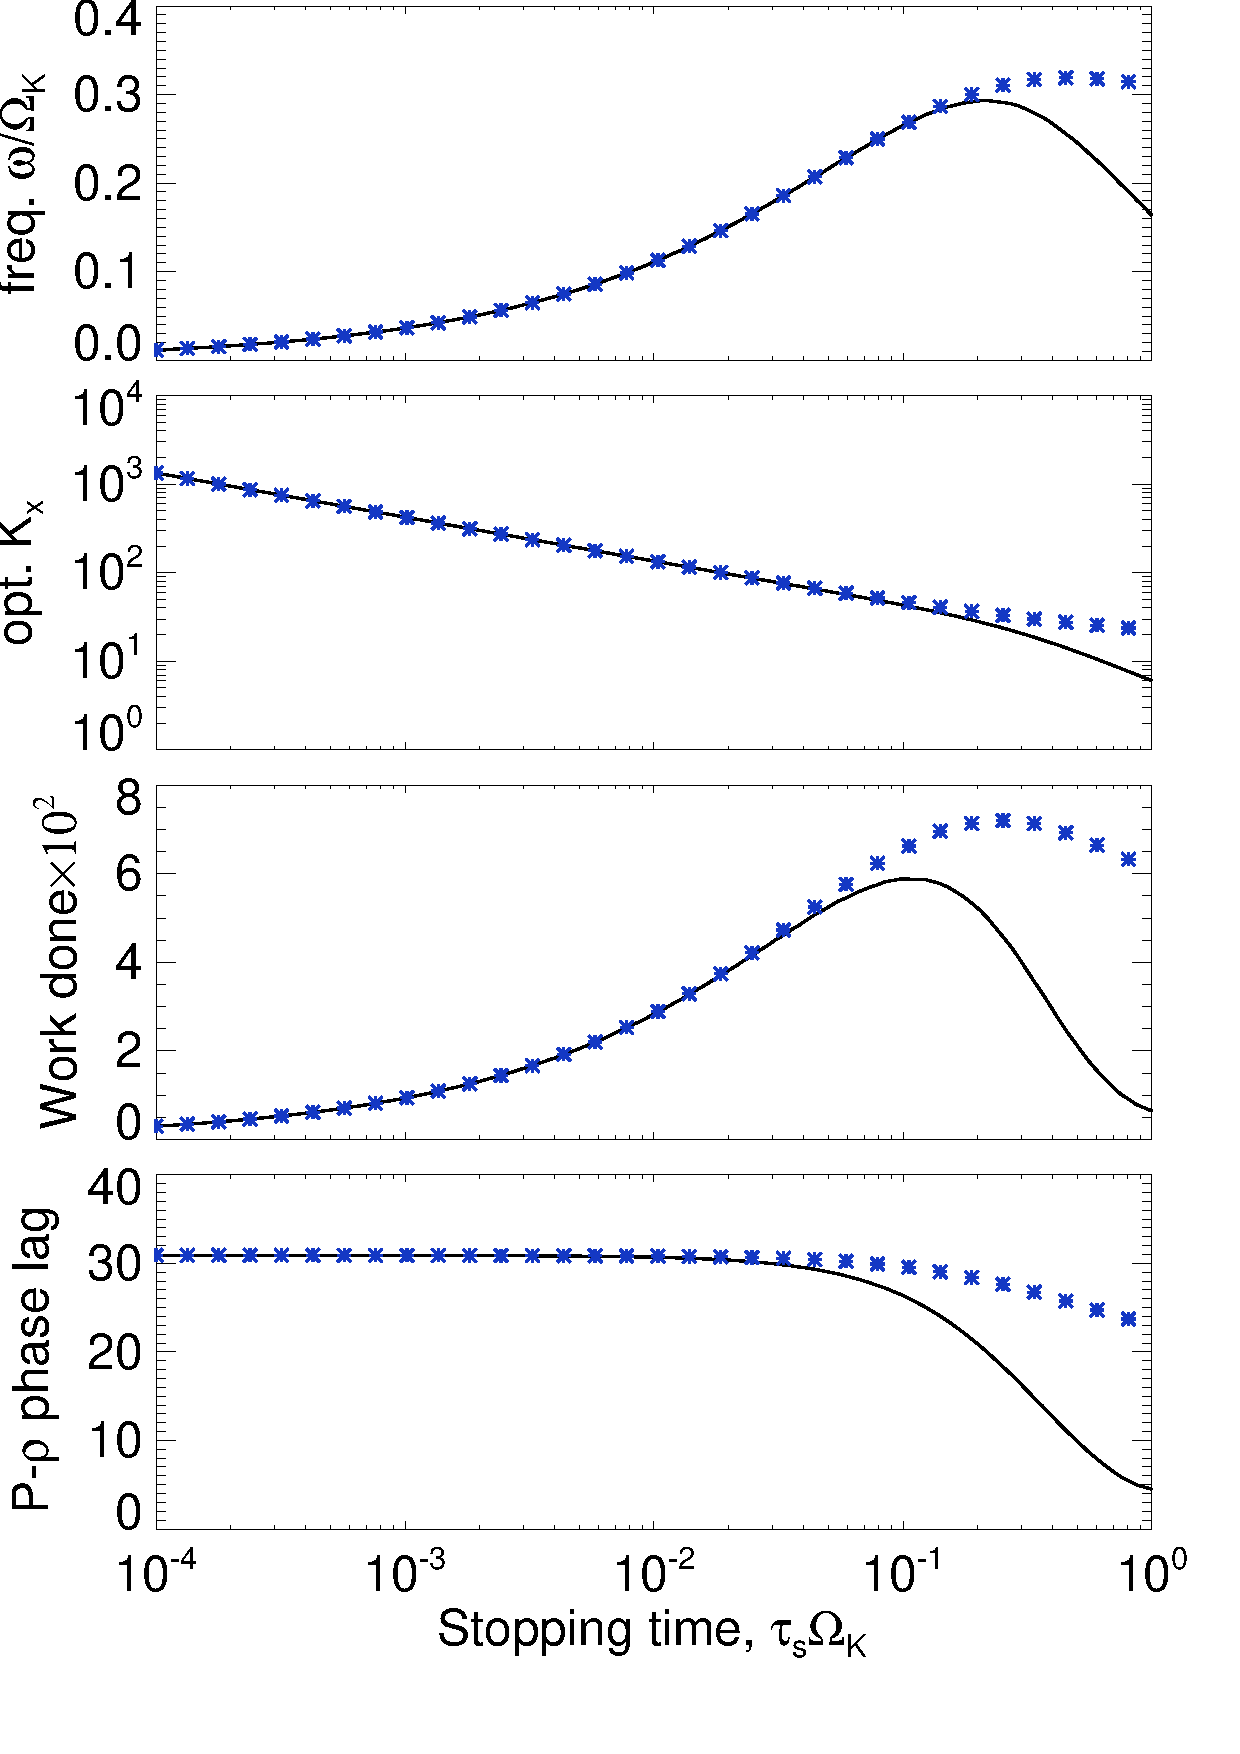
\includegraphics[width=\linewidth]{figures/si_2f_1f_compare}
\caption{Comparison of the linear 
streaming instability between a full two-fluid analysis (solid 
line), the one-fluid framework simplified by the terminal 
velocity approximation (green asterisks) and an analytic solution to
the one-fluid dispersion relation in the dust-rich limit (orange
diamonds, see also Appendix \ref{si_dust_rich}). The vertical 
wavenumber is fixed and growth rates are maximized over $K_x$. 
\label{si_compare_fig}}
\end{figure}






%"generalized stokes number" would include other problem parameters,
%e.g. wavenumber  





% \subsection{Eulerian interpretation}

% We can also consider SI in the Eulerian sense \citep[as
% did][]{jacquet11}. Eq. \ref{thermal_instability} imply SI requires
% \begin{align*}
%   \frac{\imag\left[\delta\mathcal{C}\nabla\cdot\dd\bm{v}^*\right]}{\real(\sigma)}<0. 
% \end{align*}
% The linearized dust diffusion or `cooling' term $\delta\mathcal{C}$
% for this problem is given by Eq. \ref{lin_drag_si}. Thus the
% requirement is 
% \begin{align*}
% \tepsilon |\bm{k}|^2 
%   \frac{\imag\left(\ii \sigma^* QW^*\right)}{\real(\sigma)}
% -k_x F_r\left( 1-2\tepsilon\right) 
%  | W |^2\frac{\imag\left(\sigma^*\right)}{\real(\sigma)} < 0, 
% \end{align*}
% where we have used Eq. \ref{streaming_mass}. 
% For slow growth and/or large $\left|\bm{k}\right|^2$ the second term 
% is small compared to the first. In this case instablity is due to  


%\subsection{Boundary conditions}
%Eq. \ref{lin_mass}---\ref{lin_energy} can be reduced to a set of
%first-order differential equations for $W, Q$ and $\dd v_z$. We can
%see this schematically as follows. Eq. \ref{lin_xmom} and
%\ref{lin_ymom} may be combined to yield 
%\begin{align*}
%  \dd v_r = \dd v_r (W, Q, \dd v_z). 
%\end{align*} 
%We can then take the continuity equation as an equation for $\dd v_z$, 
%\begin{align*}
%\text{Eq. \ref{lin_mass}} \Rightarrow \dd v_z^\prime(z) = \dd
%  v_z^\prime(W,Q,\dd v_z),
%\end{align*}
%and the vertical momentum equation as an equation for $Q$, 
%\begin{align*}
%\text{Eq. \ref{lin_zmom}} \Rightarrow Q^\prime(z) = 
% Q^\prime(W,Q,\dd v_z). 
%\end{align*}

%Now, for finite dust-gas coupling, $\tstop\neq0$, inspection of $\dd C$
%(Appendix \ref{lin_dust}) shows that it involves $W^\prime$ (assuming
%$\tepsilon < 1$). Then Eq. \ref{lin_energy} may be taken as a
%differential equation for $W$. However, for perfectly coupled dust,
%$\tstop =\dd\mathcal{C}= 0$. In that case Eq. \ref{lin_energy} gives an algebraic
%relation between $W$, $Q$ and $\dd v_z$. That is,
%\begin{align*}
%\text{Eq. \ref{lin_energy}}\Rightarrow \begin{cases}
%  W^\prime(z) = W^\prime(W, Q, \dd v_z) & \text{if } \tstop \neq 0, \\
%  W           (z) = W(Q, \dd v_z) & \text{if }\tstop = 0.
%\end{cases}
%\end{align*} 

%This means that for the perfectly coupled problem, we have a pair of
%ODEs for $Q$ and $\dd v_z$, and 
%When
%$\tstop\neq0$, we require three boundary conditions. {\bf WHAT?? Why odd
%  number of BCs? Shouldn't we have even number of BCs? We have
%two boundaries? I've only seen problems like this involving even
%number of BCs.} In this case we impose $\dd v_z =0$ at $z=\pm
%z_\mathrm{max}$, and classify modes according to their symmetry about
%the midplane: `even' modes with $\dd v_z^\prime(0) = 0$, and `odd' 
%modes with $\dd v_z(0)=0$.       

